\scanpage{105}
\mspage{\unsure{11|VI}}

\[
\lambda_0^{\unsure{\prime}}\quad\lambda_{1/2}\quad\lambda_1\quad\lambda_\infty
\]
\diagram{\begin{tikzcd}[ampersand replacement=\&]
\Pi'\arrow[r,phantom,"\subset"]\arrow[dr]\&\widehat{\Pi}_{0,3}\\
\&\widehat{\Pi}_{0,3}
\end{tikzcd}}

\figure{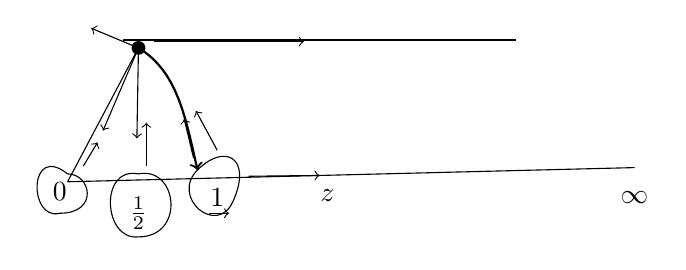
\begin{tikzpicture}[x=1cm,y=1cm]
\draw (0,0)--(7.2,.18);
\draw (.7,1.8)--(5.7,1.8);
\fill (.9,1.7) circle(2.5pt);
\draw[->] (.9,1.7)--(.45,.65);
\draw[->] (.2,.2)--(.38,.5);
\draw (.9,1.7)--(0,0);
\draw[->] (.9,1.7)--(.88,.55);
\draw[->] (1,.2)--(1,.75);
\draw[thick,->] (.9,1.7) .. controls (1.4,1.4) and (1.5,.8) .. (1.65,.15);
\draw[->] (1.6,.3)--(1.48,.8);
\draw[->] (1.9,.4)--(1.63,.9);
\draw (0,.1) .. controls (-.5,.5) and (-.5,-.5) .. (-.1,-.4)
 .. controls (.4,-.4) and (.3,.1) .. (0,.1);
\draw (.9,.1) .. controls (.4,.2) and (.45,-.75) .. (.9,-.7)
 .. controls (1.5,-.7) and (1.4,.2) .. (.9,.1);
\draw (1.65,.15) .. controls (2,.5) and (2.35,.3) .. (2.1,-.25)
 .. controls (1.9,-.7) and (1.3,-.2) .. (1.65,.15);
\draw[->] (.9,1.7)--(.3,1.95);
\draw[->] (1.1,1.78)--(3,1.78);
\draw[->] (2.3,.07)--(3.2,.08);
\draw[->] (1.8,-.4)--(2.05,-.4);
\node at (-.1,-.12) {$0$};
\node at (.9,-.4) {$\frac12$};
\node at (1.9,-.2) {$1$};
\node at (3.3,-.18) {\deleted{$\unsure{z}$}};
\node at (7.2,-.2) {$\infty$};
\end{tikzpicture}}

\[
(-2\bar j-1)^2=4\bar j^{\,2}+
\]

\diagram{\begin{tikzcd}[ampersand replacement=\&]
\lambda_{\unsure{1/2|d/2}}^{\unsure{k}}\arrow[r,"\deleted{\unsure{\zeta}}"]\&l_0
\end{tikzcd}}
\deleted{$2z-1$}\quad$\lambda$

\figure{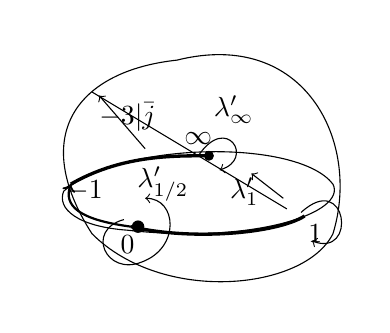
\begin{tikzpicture}[x=1cm,y=1cm,scale=.9]
\draw (0,.2) .. controls (-.9,1.6) and (-.2,2.5) .. (1.2,2.65)
 .. controls (3,3.1) and (3.8,1.5) .. (3.4,.2)
 .. controls (3,-.6) and (1,-.8) .. (0,.2);
\draw (-.4,.8) .. controls (.4,1.5) and (2.9,1.55) .. (3.4,.9)
 .. controls (3.6,.5) and (2.3,.05) .. (.5,.25)
 .. controls (-.2,.3) and (-.5,.55) .. (-.4,.8);
\draw[very thick] (.55,.3) .. controls (1.4,.1) and (2.6,.2) .. (3,.45);
\draw[thick,->] (.55,.3) .. controls (-.2,.4) and (-.4,.6) .. (-.3,.9);
\draw[very thick] (-.3,.9) .. controls (.4,1.3) and (1.1,1.3) .. (1.6,1.3);
\draw (0,2.2)--(2.75,.55);
\draw[->] (2.7,.7)--(2.25,1.05);
\draw[->] (.75,1.4)--(.1,2.15);
\fill (.65,.3) circle(2.5pt);
\fill (1.65,1.3) circle(2pt);
\draw[->] (.45,.4) .. controls (-.1,.25) and (.2,-.4) .. (.7,-.2)
 .. controls (1.25,0) and (1.2,.7) .. (.75,.7);
\draw[->] (2.95,.5) .. controls (3.6,1.1) and (3.75,-.15) .. (3.1,.1);
\draw[->] (1.5,1.3) .. controls (1.9,1.9) and (2.3,1.25) .. (1.8,1.1);
\node at (-.1,.8) {$-1$};
\node at (.5,1.85) {$-\unsure{3|\bar j}$};
\node at (1.5,1.55) {$\infty$};
\node at (.5,.05) {$0$};
\node at (3.15,.2) {$1$};
\node at (1,.9) {$\lambda'_{1/2}$};
\node at (2.15,.8) {$\lambda'_1$};
\node at (2,1.95) {$\lambda'_\infty$};
\end{tikzpicture}
\qquad
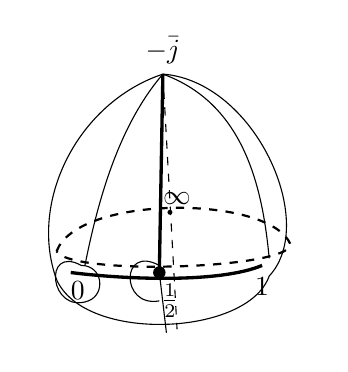
\begin{tikzpicture}[x=1cm,y=1cm,scale=.9]
\draw (0,0) .. controls (-.4,1.1) and (.3,2.5) .. (1.5,2.9)
 .. controls (2.8,2.8) and (3.7,.8) .. (3,.05)
 .. controls (2.7,-.8) and (.4,-.9) .. (0,0);
\draw[dashed,thick] (0,.4) .. controls (.3,1.2) and (3,1.2) .. (3.3,.5)
 .. controls (3.3,.15) and (.2,.05) .. (0,.4);
\draw[very thick] (.2,.1) .. controls (1,.0) and (2.3,-.05) .. (2.9,.2);
\draw[very thick] (1.5,2.9)--(1.45,.1);
\draw (.4,.2) .. controls (.6,1.2) and (.9,2.2) .. (1.5,2.9);
\draw (1.5,2.9) .. controls (2.6,2.5) and (2.9,1.4) .. (3,.3);
\draw[dashed] (1.5,2.9)--(1.7,-.7);
\draw (1.45,.1)--(1.55,-.75);
\draw (.35,.2) .. controls (-.2,.5) and (-.1,-.5) .. (.45,-.3)
 .. controls (.7,-.2) and (.65,.2) .. (.35,.2);
\draw (1.45,.2) .. controls (.9,.5) and (.9,-.4) .. (1.45,-.3);
\fill (1.45,.1) circle(2.5pt);
\fill (1.6,.95) circle(1pt);
\node[above] at (1.5,2.9) {$-\bar j$};
\node at (.3,-.15) {$0$};
\node at (2.9,-.1) {$1$};
\node at (1.6,-.3) {$\frac12$};
\node at (1.7,1.15) {$\infty$};
\end{tikzpicture}
\qquad
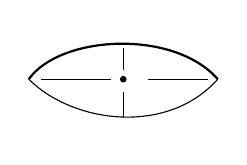
\begin{tikzpicture}[scale=.8]
\draw[thick] (0,0) .. controls (.5,.7) and (2.3,.8) .. (3,0);
\draw (0,0) .. controls (.7,-.7) and (2.2,-.9) .. (3,0);
\fill (1.5,0) circle(1.5pt);
\draw (.2,0)--(1.3,0);
\draw (1.9,0)--(2.85,0);
\draw (1.5,.15)--(1.5,.5);
\draw (1.5,-.2)--(1.5,-.6);
\end{tikzpicture}}

\deleted{$2z-1$}
\[
(2x-1+2iy)^2=(2x-1)^2-4y^2+4iy(2x-1)
\]
\[
y=0\qquad x=\tfrac12
\]

\deleted{$\dot{\sigma}_\infty(z)=1-z$}
\[
(-2\bar j+1)^2=4\bar j^{\,2}+1-4\bar j=4(\bar j^{\,2}-\bar j)
\]
\deleted{$\unsure{u}\mathbin{-}\unsure{\lambda}$}
\deleted{$\zeta^2-\zeta+1$}

\[
(2\zeta-1)^2=4\underbrace{(\zeta^2-\zeta)}_{-1}+1=-3
\]
\[
\zeta^2-\zeta+1=(\zeta-\alpha)(\zeta-\unsure{\bar\alpha|\bar\varphi})
\]
\deleted{$\alpha\mathbin{\unsure{+|\cdot}}\bar\alpha=1$}

\diagram{\begin{tikzcd}[ampersand replacement=\&]
\lambda_0\arrow[r,maps to]\&
\deleted{(l_\infty^2l_1l_0^2)^{-1}}
=l_0^{-2}l_1^{-1}l_\infty^{-2}
\end{tikzcd}}
\[
=l_0^{-1}l_\infty^{-1}=l_0^{-1}l_1l_0
\]
\diagram{\begin{array}{c}
\begin{tikzcd}[ampersand replacement=\&,row sep=small]
\lambda_{1/2}\arrow[r,maps to]\&l_0^{2\unsure{k}}\\
\lambda_1\arrow[r,maps to]\&l_1\\
\lambda_\infty\arrow[r]\&l_\infty^2
\end{tikzcd}\ \left.\vphantom{\begin{matrix}l_0^{2k}\\l_1\\l_\infty^2\end{matrix}}\right\}
\end{array}}

\deleted{$\begin{aligned}
&=(l_\infty l_0)^{-1}\\
&=\bigl(\operatorname{int}(l_0^{-1})\bigl((l_0l_\infty)^{\unsure{*}}\bigr)\bigr)^{-1}\\
&=\operatorname{int}(l_0^{-1})\bigl(\underbrace{(l_0l_\infty)^{-1}}_{l_1}\bigr)
\end{aligned}$}
\[
=\operatorname{int}(l_0^{-1})(l_1)
\]
\deleted{$l_0^{-1}l_1l_0$}
\deleted{$\begin{aligned}
l_1l_0l_\infty&=1\\
l_1^{-1}&=l_0l_\infty\\
l_1&=l_\infty^{-1}l_0^{-1}
\end{aligned}$}

\[
l_0^{-1}(l_0l_\infty\quad l_0
\]
\deleted{$ab\unsure{=}(a^{-1}b^{-1})(ba)ab$}

\margin{104}
